\documentclass[a4paper]{article}

% {{{ [begin] thai language support
% http://thaitug.daytag.org/wordpress/?p=1947
\usepackage{fontspec}
\usepackage{polyglossia}
\usepackage[Latin,Thai]{ucharclasses}
\defaultfontfeatures{Mapping=tex-text} 
\setdefaultlanguage{thai}
\setotherlanguage{english}
\newfontfamily{\thaifont}[Scale=MatchUppercase,Mapping=tex-text]{Norasi:script=thai}
\setTransitionTo{Thai}{\thaifont}
\setTransitionFrom{Thai}{\normalfont}
\XeTeXlinebreaklocale “th_TH” 
\XeTeXlinebreakskip = 0pt plus 1pt
\linespread{1.5}
% }}} [end] thai language support

\usepackage[hidelinks]{hyperref} % external URL clickable link without
                                 % visible box around the link
\usepackage{fancybox} % "Do you know?" box

% file path formatting
\usepackage{url}
\renewcommand\UrlFont{\thaifont\itshape}

% source code formatting
\usepackage{listings}
% {{{
\usepackage{color}
\definecolor{dkgreen}{rgb}{0,0.6,0}
\definecolor{gray}{rgb}{0.5,0.5,0.5}
\definecolor{mauve}{rgb}{0.58,0,0.82}
\lstset{frame=tb,
  language=Java,
  aboveskip=3mm,
  belowskip=3mm,
  showstringspaces=false,
  columns=flexible,
  basicstyle={\small},
  numbers=none,
  numberstyle=\tiny\color{gray},
  keywordstyle=\color{blue},
  commentstyle=\color{dkgreen},
  stringstyle=\color{mauve},
  breaklines=true,
  breakatwhitespace=true,
  tabsize=3
}

\lstset{numbers=left,numberstyle=\tiny,numbersep=5pt,language=Lisp,
  stringstyle=\small,basicstyle=\footnotesize,
  showstringspaces=false,breaklines}
% }}}

\usepackage{xcolor,graphicx}

\usepackage{p4bwcl} % my package

\begin{document}

\title{Programming For Beginners With Common~Lisp}
\author{unsigned\_nerd}
\maketitle

\tableofcontents

\section{การเริ่มต้น}

การเขียนโปรแกรม คือ การเขียนชุดคำสั่งเพื่อสั่งให้คอมพิวเตอร์ทำงานตามที่เรากำหนด

เราเขียนชุดคำสั่งด้วย Programming Language

โดยทั่วไปหากเราพูดถึง Programming Language เราจะหมายถึงภาษาแบบ High-Level เช่น
Common Lisp, Python, Java, PHP, Perl, C, JavaScript เป็นต้น
แต่ไม่ได้หมายถึงภาษา Assembly\footnote{ภาษา Assembly เป็น Low-Level
Programming Language}

ภาษา Common Lisp เป็นภาษาที่ปัจจุบันไม่ได้รับความนิยมเลยทั้งๆที่มี Feature ต่างๆมากมาย 
โดยเฉพาะอย่างยิ่ง Macro ใน Common Lisp ที่ทำให้เราสามารถเพิ่ม Syntax ต่างๆที่%
ต้องการเองได้ ทำให้เราสามารถเขียนโค้ดที่มีความกระชับและสั้นได้ง่าย\footnote{การเขียนโค้ด
หากเขียนได้ยิ่งสั้นก็ถือว่ายิ่งดี โค้ดที่สั้นย่อมมีโอกาสเกิด Bug ได้น้อยกว่าโค้ดที่ยาว
อีกทั้งยังสามารถอ่านได้เข้าใจได้ง่ายกว่าอีกด้วย ท่านคงเคยได้ยินคำกล่าวที่ว่า การเขียน
Function ใดๆ ไม่ควรเขียนให้มีความยาวเกินความสูงของหน้าจอคอมฯของท่าน} ตัวอย่างเช่น
หากเราต้องการเขียนโปรแกรมที่ทำการอ่านข้อมูลแบบ Plain Text จาก Standard Input
แล้วทำการใส่ Prefix String "Common Lisp is fun?: " นำหน้าทุกบรรทัด
ก่อนที่จะพิมพ์ข้อมูลในแต่ละบรรทัดออกไปยัง Standard Output โดยปกติเราอาจเขียนโค้ดดังนี้:

\lstset{language=Lisp}
\begin{lstlisting}
(let (line)
  (loop for line = (read-line *standard-input* nil 'eof)
    until (eq line 'eof)
    do
      (format t "Common Lisp is fun?  ~A~%" line)))
\end{lstlisting}

ซึ่งจะเห็นได้ว่ามันดูเข้าใจยากและรายละเอียดเยอะไปหมด ทั้ง loop, until, do, 'eof และ
nil แต่หากเราเขียน Macro ดังนี้:

\lstset{language=Lisp}
\begin{lstlisting}
(defmacro for-each-$line-in (in-stream &rest body)
  (let (($line (intern (symbol-name '$line))))
    `(let (,$line)
       (loop for ,$line = (read-line ,in-stream nil 'eof)
         until (eq ,$line 'eof)
         do
           ,@body))))
\end{lstlisting}

ซึ่งจะเห็นได้ว่าเป็นเพียงการลอกโค้ดที่เราเขียนไว้ก่อนหน้ามาสร้างเป็น Macro\footnote{ซึ่ง%
อ่านเข้าใจยากกว่าเก่า แต่โดยปกติ Macro จะอยู่ในลักษณะของ Package ให้เราเรียกใช้
เราจึงไม่ต้องอ่านโค้ดที่ซับซ้อนเหล่านี้เวลาใช้งาน} จะทำให้เรา%
สามารถเขียนโค้ดใหม่ได้ดังนี้:

\lstset{language=Lisp}
\begin{lstlisting}
(for-each-$line-in *standard-input*
  (format t "Common Lisp is fun?  ~A~%" $line))
\end{lstlisting}

ซึ่งสั้นกว่าเดิมมาก

ท่านผู้อ่านที่ยังไม่รู้ว่า Macro คืออะไรอาจจะเห็นโค้ดนี้แล้วเห็นว่าสามารถใช้การเขียน Function 
ทำได้เหมือนกัน ซึ่งหากลองเพ่งดูดีๆจะพบว่าไม่สามารถทำได้ โดยมีจุดที่น่าสังเกตดังนี้

\begin{enumerate}
  \item a
  \item b
\end{enumerate}

สามารถดูการจัดอันดับภาษาคอมฯที่ได้รับความนิยมล่าสุดได้ที่นี่: \href{http://pypl.github.io/PYPL.html}{http://pypl.github.io/PYPL.html}

อันดับหนึ่งคือภาษา Python ส่วนภาษา Common Lisp ไม่ติดอันดับบน PYPL เลย

ทาง PYPL แนะนำว่าถ้าหากอยากทราบความนิยมของภาษาที่ไม่ติดอันดับให้ใช้ Google Trends ดู

เมื่อลองใช้ Google Trends เปรียบเทียบความนิยมระหว่าง 3 ภาษา ได้แก่ Python, PHP
และ Common Lisp เราจะพบว่ากระแสความนิยมในภาษา Common Lisp นั้นต่ำมาก
ดังจะเห็นได้จากรูปที่ \ref{lang-pop}:

\begin{figure}[!hbtp]
  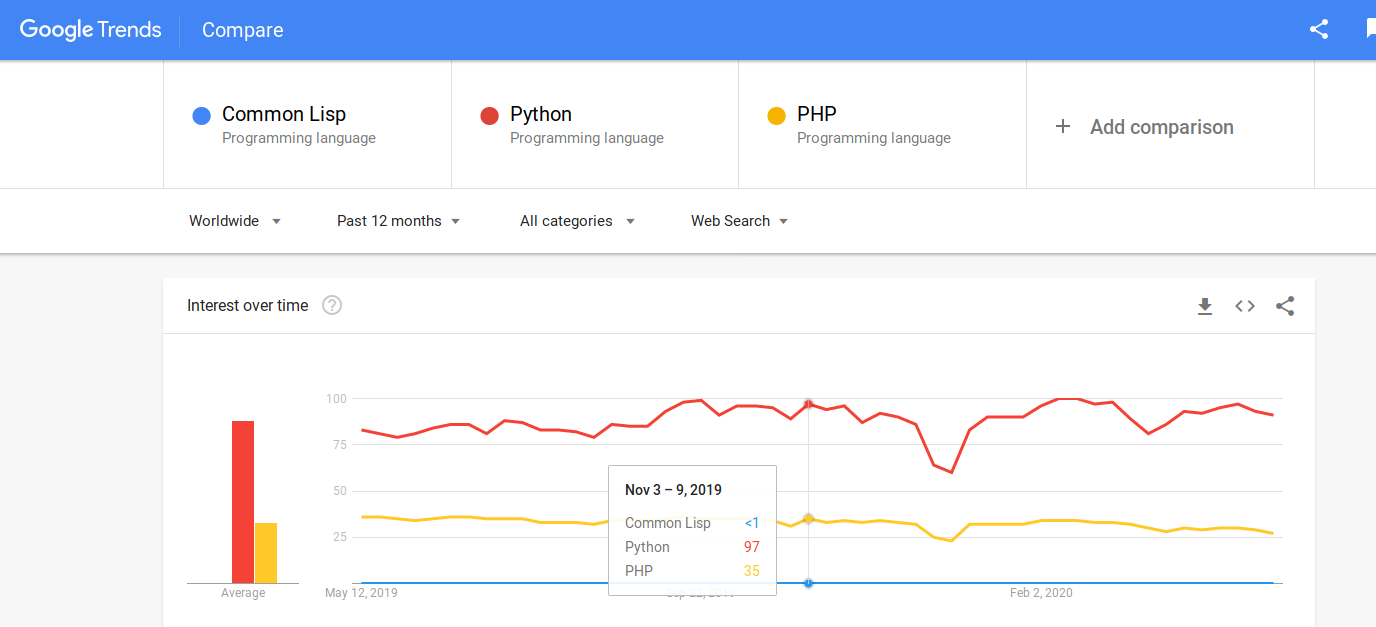
\includegraphics[width=\linewidth]{images/lang-popularity.png}
  \caption{Language popularity\label{lang-pop}}
\end{figure}

อย่างไรก็ตาม แม้ว่า Common Lisp จะไม่ได้รับความนิยมในปัจจุบัน
แต่ก็ไม่ได้หมายความว่ามันจะไม่เหมาะกับการใช้เป็นเครื่องมือในการเรียนรู้การเขียนโปรแกรม%
สำหรับมือใหม่

เมื่อท่านได้เรียนรู้การเขียนโปรแกรมด้วยภาษา Common Lisp แล้ว ท่านจะสามารถเรียนภาษา%
คอมฯอื่นๆเพิ่มเติมได้ง่ายขึ้นมาก

เป็นที่ยอมรับกันโดยทั่วไปว่าในชีวิตหนึ่งๆของคนเรา เราย่อมต้องเรียนภาษาคอมพิวเตอร์หลาย%
ภาษากันอยู่แล้ว แล้วทำไมจึงไม่ลองเรียนภาษา Common Lisp กันเล่า!

\doyouknow{
  ภาษา Logo (เจ้าเต่าน้อย Logo) ที่หลายๆท่านอาจได้เคยเรียนในสมัยเด็กๆเป็น
    Dialect หนึ่งของภาษา Lisp นี่ก็ยิ่งชี้ให้เห็นว่า Common Lisp
    เหมาะกับการเป็นภาษาเขียนโปรแกรมแรกๆของทุกท่านขนาดไหน
}

\section{Common Lisp Package, ASDF, System และ Quicklisp}

เรื่อง Package, ASDF, System และ Quicklisp
เป็นเรื่องหนึ่งที่ผู้เขียนมีความสับสนมากในช่วงเริ่มต้นของการเรียนภาษา Common Lisp

ความยืดหยุ่นที่มากเกินไป กับ Documentation ที่ไม่ดีนักก็ทำให้เกิดผลเสียต่อความนิยมของภาษา%
คอมฯหนึ่งๆได้

เรื่องนี้เกี่ยวกับระบบ Software Library ใน Common Lisp

สำหรับมือใหม่ ให้ลองทำตามนี้ก่อน จะได้ไม่สับสน แล้วเมื่อเชี่ยวชาญแล้วค่อยปรับแต่งตามใจชอบ

Software Library ต่างๆใน Common Lisp จะอยู่ในสิ่งที่เรียกว่า System

System หนึ่งๆจะประกอบไปด้วย Package ตั้งแต่ 1 อันขึ้นไป โดยจะใช้ ASDF เป็นตัวบอก%
ว่าไฟล์ต่างๆของ Package ทั้งหลายน้้นอยู่ตรงไหน


เวลาเราจะเปิด Project ใหม่ สมมุติว่าชื่อ hello-world ให้เราไปที่ Directory ชื่อ
\path{~/common-lisp/} แล้วสร้าง directory ชื่อ \path{hello-world/} ขึ้นมา
ซึ่งจะเป็นที่ๆเราจะใส่ Source Code ของเราในนั้น

ต่อมาเรามี Project ใหม่ สมมุติว่าชื่อ goodbye-universe เราก็สร้าง Directory ชื่อ
\path{~/common-lisp/goodbye-universe/} แล้วใส่ Source Code ของ Project
นี้ไปในนั้น

สมมุติว่าเรามี Function ใน Project ชื่อ hello-world ที่สามารถนำมาใช้ใน Project ชื่อ
goodbye-universe ด้วย ทางหนึ่งที่ทำได้คือ Copy \& Paste Source Code ของ
Function นั้นมาใส่ แต่วิธีนี้ไม่ดี

วิธีที่ดีกว่าคือ เอา Function นั้นไปสร้างเป็น Package แล้วให้ Project ชื่อ
hello-world และ goodbye-universe เรียกใช้ Function นั้นร่วมกันผ่านระบบ Package

เมื่อเราจัดเอา Function และ/หรือ โค้ดส่วนอื่นๆที่สามารถใช้ร่วมกันได้ระหว่างหลาย
Project มาจัดใส่ Package ต่างๆแล้ว เราก็ต้องมาคิดต่อว่าจะต้องทำอย่างไร Sbcl จึงจะรู้%
ว่าไฟล์ Package ต่างๆอยู่ที่ไหน ซึ่งนี่จะเป็นหน้าที่ของ ASDF

ASDF คือเครื่องมือที่จะบอก Sbcl ว่าไฟล์ต่างๆอยู่ตรงไหน


\section{การติดตั้งระบบเพื่อเริ่มเขียนโปรแกรมด้วยภาษา Common Lisp}

Common Lisp มีหลาย Implementation เราเลือกใช้ Sbcl ซึ่งเป็น Common Lisp Implementation ที่ได้รับความนิยมที่สุด

ผู้เขียนใช้ Debian 10 เป็น Operating System

ทำการติดตั้ง Sbcl, Quicklisp และ un-utils บนคอมฯของท่านโดยทำตามขั้นตอนในลิงค์นี้:
\href{https://github.com/unsigned-nerd/un-utils}{https://github.com/unsigned-nerd/un-utils}

Sbcl

ดังได้กล่าวไปก่อนหน้านี้ Sbcl เป็น Implementation หนึ่งของ Common Lisp

เป็นโปรแกรมที่ใช้คอมไพล์และรันโปรแกรมที่เราเขียนขึ้นด้วยภาษา Common Lisp

Quicklisp

Quicklisp เป็นโปรแกรมเชิงระบบที่นิยมใช้ในการติดตั้ง Systems ต่างๆจากผู้พัฒนาคนอื่น

System ใน Common Lisp ก็คือ Library ต่างๆที่เราเรียกกันในภาษาอื่นนั่นเอง

โดยทั่วไป ให้เราคิดเสียว่า หากเราต้องการดาวน์โหลด System ของคนอื่นมาใช้
โดยคิดว่าจะใช้อย่างเดียว ไม่ได้ต้องการจะแก้ไขอะไรมัน ก็ควรจะใช้ Quicklisp
ในการดาวน์โหลดและติดตั้ง

แต่ถ้าเราต้องการเขียน System เอง หรือ ต้องการแก้ไข System ของผู้อื่น ก็ให้ใช้เครื่องมือชื่อ
ASDF ในการจัดการ

ASDF เป็นเครื่องมือที่ใช้ในการจัดการ

un-utils

un-utils เป็น Common Lisp System ที่ทางผู้เขียนพัฒนาขึ้นมา ซึ่งมี Package ที่น่าสนใจชื่อ
un-utils.simple-syntax

un-utils.simple-syntax นี้จะ

\lstset{language=Java}
\begin{lstlisting}
// Hello.java
import javax.swing.JApplet;
import java.awt.Graphics;

public class Hello extends JApplet {
    public void paintComponent(Graphics g) {
        g.drawString("Hello, world!", 65, 95);
    }    
}
\end{lstlisting}

\lstset{language=Lisp}
\begin{lstlisting}
; comment
(setf a 'a)
\end{lstlisting}


\end{document}

% todo
%
% - what other langs have
%   - list comprehension in python
%   - with statement
%
